\section{Experiments and Evaluation}
\frame{\tableofcontents[currentsection]}


\begin{frame}
    \frametitle{Cost Function Evaluation (3x15 points, $\noise=1$)}
    % blue and red dots distributed on the y-axis,
    % conflicts and and their bad effect on the partial optimality
    \begin{figure}[h]
        \centering
        \vspace{-10px}
        \begin{minipage}{0.17\textwidth}
            \textbf{Blue:}\\ 
            same\\
            plane
            
            \vspace{15px}
            \textbf{Red:}\\
            different\\
            planes
        \end{minipage}
        \begin{minipage}{0.8\textwidth}
            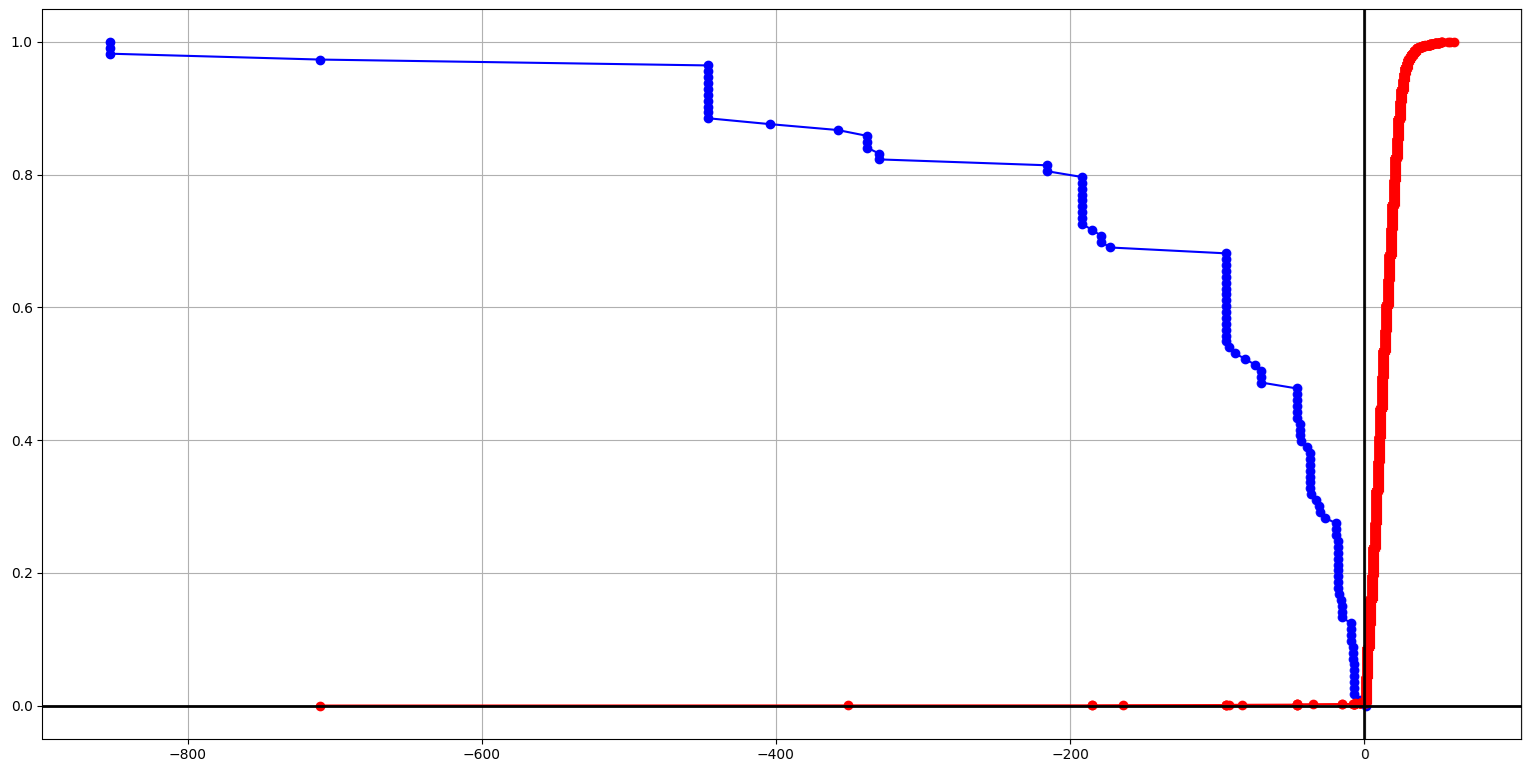
\includegraphics[width=\textwidth]{c-eval-big.png}
        \end{minipage}
        \onslide<2->{
        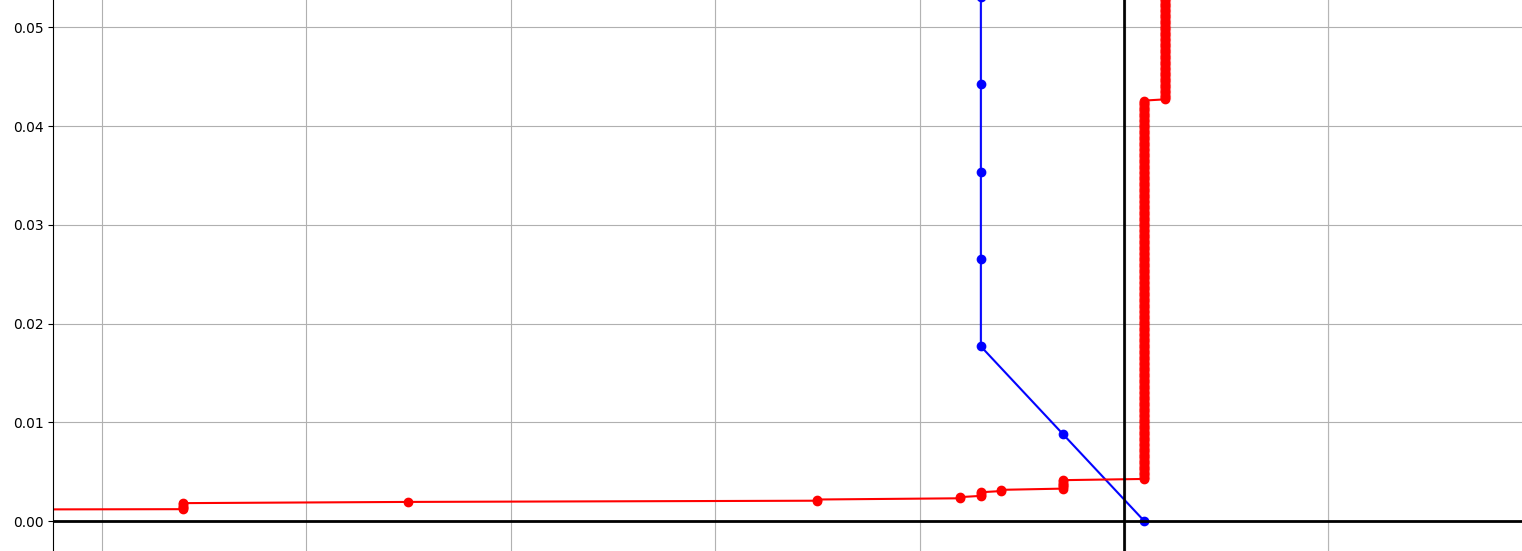
\includegraphics[width=\textwidth]{c-eval-little.png}
        }
        \vspace{-15px}
    \end{figure}
\end{frame}


\begin{frame}
    \frametitle{Experiments}
    \begin{itemize}
        \onslide<1->{
        \item WSL2 Ubuntu,
        Intel Core i7-11370H (3.30 GHz), 
        16 GB RAM} \onslide<2->{ 
        \item Apply the algorithm to the random cubic subspace instances\\
        with $\maxD=100$ and fixed $\noise=0,1,2,3,4,5$:
        \begin{itemize}
            \item 3x7 points (solve 15 instances)
            \item 3x10 points (solve 15 instances)
            \item 3x15 points (solve 7 instances)
            \item 3x20 points (solve 1 instance)
        \end{itemize}
        } \onslide<3->{
        \item Track
        \begin{itemize}
            \item computation time (s)
            \item partial optimality (\%)
            \item accuracy (\%) with respect to the truth (correct labeling)
        \end{itemize}
        } \onslide<4->{
        \item Capture
        \begin{itemize}
            \item 1.quartile (Q1)
            \item median (Q2)
            \item 3.quartile(Q3)
            \item the worst computation time
        \end{itemize}
        }
    \end{itemize}
\end{frame}




\begin{frame}
    \frametitle{Partial Optimality / Accuracy (3x7 points)}
    % not enough information to join all the same plane points!
    % losing partial optimality because of conflicts!
    \resizebox{0.95\textwidth}{!}{
    \begin{tikzpicture}
        \begin{axis}[
            legend style={font=\tiny},
            xlabel=$\noise$, ylabel=Partial Optimality / Accuracy,
            xmin=0, xmax=5,
            ymin=0, ymax=1,
            grid=major,
            legend style={
                at={(0.35,0)},
                anchor=south east
            },
            every axis plot/.append style={line width=1.5pt}
        ]
            \addplot[color=lightblue] table[x=noise, y=opt_q1, col sep=comma] {data7_of_noise.csv};
            \addlegendentry{part.opt.Q1}
            \addplot[color=blue, line width=3pt] table[x=noise, y=opt_med, col sep=comma] {data7_of_noise.csv};
            \addlegendentry{part.opt.Q2}
            \addplot[color=darkblue] table[x=noise, y=opt_q3, col sep=comma] {data7_of_noise.csv};
            \addlegendentry{part.opt.Q3}
            \addplot[color=lightred] table[x=noise, y=acc_q1, col sep=comma] {data7_of_noise.csv};
            \addlegendentry{accuracy Q1}
            \addplot[color=red, line width=3pt] table[x=noise, y=acc_med, col sep=comma] {data7_of_noise.csv};
            \addlegendentry{accuracy Q2}
            \addplot[color=darkred] table[x=noise, y=acc_q3, col sep=comma] {data7_of_noise.csv};
            \addlegendentry{accuracy Q3}
        \end{axis}
    \end{tikzpicture}
    }
\end{frame}

\begin{frame}
    \frametitle{Partial Optimality / Accuracy (3x10 points)}
    % higher accuracy, but losing partial optimality because of conflicts
    \resizebox{0.95\textwidth}{!}{
    \begin{tikzpicture}
        \begin{axis}[
            legend style={font=\tiny},
            xlabel=$\noise$, ylabel=Partial Optimality / Accuracy,
            xmin=0, xmax=5,
            ymin=0, ymax=1,
            grid=major,
            legend style={
                at={(1,0.2)},
                anchor=south east
            },
            every axis plot/.append style={line width=1.5pt}
        ]
            \addplot[color=lightblue] table[x=noise, y=opt_q1, col sep=comma] {data10_of_noise.csv};
            \addlegendentry{part.opt.Q1}
            \addplot[color=blue, line width=3pt] table[x=noise, y=opt_med, col sep=comma] {data10_of_noise.csv};
            \addlegendentry{part.opt.Q2}
            \addplot[color=darkblue] table[x=noise, y=opt_q3, col sep=comma] {data10_of_noise.csv};
            \addlegendentry{part.opt.Q3}
            \addplot[color=lightred] table[x=noise, y=acc_q1, col sep=comma] {data10_of_noise.csv};
            \addlegendentry{accuracy Q1}
            \addplot[color=red, line width=3pt] table[x=noise, y=acc_med, col sep=comma] {data10_of_noise.csv};
            \addlegendentry{accuracy Q2}
            \addplot[color=darkred] table[x=noise, y=acc_q3, col sep=comma] {data10_of_noise.csv};
            \addlegendentry{accuracy Q3}
        \end{axis}
    \end{tikzpicture}
    }
\end{frame}

\begin{frame}
    \frametitle{Partial Optimality / Accuracy (3x15 points)}
    % even higher accuracy, but losing partial optimality because of too many conflicts!
    \resizebox{0.95\textwidth}{!}{
    \begin{tikzpicture}
        \begin{axis}[
            legend style={font=\tiny},
            xlabel=$\noise$, ylabel=Partial Optimality / Accuracy,
            xmin=0, xmax=5,
            ymin=0, ymax=1,
            grid=major,
            legend style={
                at={(1,0.2)},
                anchor=south east
            },
            every axis plot/.append style={line width=1.5pt}
        ]
            \addplot[color=lightblue] table[x=noise, y=opt_q1, col sep=comma] {data15_of_noise.csv};
            \addlegendentry{part.opt.Q1}
            \addplot[color=blue, line width=3pt] table[x=noise, y=opt_med, col sep=comma] {data15_of_noise.csv};
            \addlegendentry{part.opt.Q2}
            \addplot[color=darkblue] table[x=noise, y=opt_q3, col sep=comma] {data15_of_noise.csv};
            \addlegendentry{part.opt.Q3}
            \addplot[color=lightred] table[x=noise, y=acc_q1, col sep=comma] {data15_of_noise.csv};
            \addlegendentry{accuracy Q1}
            \addplot[color=red, line width=3pt] table[x=noise, y=acc_med, col sep=comma] {data15_of_noise.csv};
            \addlegendentry{accuracy Q2}
            \addplot[color=darkred] table[x=noise, y=acc_q3, col sep=comma] {data15_of_noise.csv};
            \addlegendentry{accuracy Q3}
        \end{axis}
    \end{tikzpicture}
    }
\end{frame}

\begin{frame}
    \frametitle{Partial Optimality (Q1)}
    % 1.quartile: partial optimality loss is even more noticable
    \resizebox{0.9\textwidth}{!}{
    \begin{tikzpicture}
        \begin{axis}[
            xlabel=\#points/3, ylabel=Partial Optimality,
            xmin=7, xmax=15,
            ymin=0, ymax=1,
            grid=major,
            legend style={
                at={(0.95,0.4)},
                anchor=south east
            },
            every axis plot/.append style={line width=3pt}
        ]
            \addplot[color=blue, mark=*] table[x=n, y=opt_q1_noise0, col sep=comma] {data_of_size.csv};
            \addlegendentry{$\noise = 0$}
            \addplot[color=warmorange, mark=*] table[x=n, y=opt_q1_noise1, col sep=comma] {data_of_size.csv};
            \addlegendentry{$\noise = 1$}
            \addplot[color=forestgreen, mark=*] table[x=n, y=opt_q1_noise2, col sep=comma] {data_of_size.csv};
            \addlegendentry{$\noise = 2$}
        \end{axis}
    \end{tikzpicture}
    }
\end{frame}

\begin{frame}
    % partial optimality for different point counts and different noises 
    % noise tolerance up to 3 percents!!!
    \frametitle{Partial Optimality (Q2)}
    \resizebox{0.9\textwidth}{!}{
    \begin{tikzpicture}
        \begin{axis}[
            xlabel=\#points/3, ylabel=Partial Optimality,
            xmin=7, xmax=15,
            ymin=0, ymax=1,
            grid=major,
            legend style={
                at={(0.95,0.2)},
                anchor=south east
            },
            every axis plot/.append style={line width=3pt}
        ]
            \addplot[color=blue, mark=*] table[x=n, y=opt_med_noise0, col sep=comma] {data_of_size.csv};
            \addlegendentry{$\noise = 0$}
            \addplot[color=warmorange, mark=*] table[x=n, y=opt_med_noise1, col sep=comma] {data_of_size.csv};
            \addlegendentry{$\noise = 1$}
            \addplot[color=forestgreen, mark=*] table[x=n, y=opt_med_noise2, col sep=comma] {data_of_size.csv};
            \addlegendentry{$\noise = 2$}
        \end{axis}
    \end{tikzpicture}
    }
\end{frame}

\begin{frame}
    \frametitle{Partial Optimality (Q3)}
    % 3.quartile:for some generated instances, the partial optimality can still be kept at pretty high level
    \resizebox{0.9\textwidth}{!}{
    \begin{tikzpicture}
        \begin{axis}[
            xlabel=\#points/3, ylabel=Partial Optimality,
            xmin=7, xmax=15,
            ymin=0, ymax=1,
            grid=major,
            legend style={
                at={(0.95,0.6)},
                anchor=south east
            },
            every axis plot/.append style={line width=3pt}
        ]
            \addplot[color=blue, mark=*] table[x=n, y=opt_q3_noise0, col sep=comma] {data_of_size.csv};
            \addlegendentry{$\noise = 0$}
            \addplot[color=warmorange, mark=*] table[x=n, y=opt_q3_noise1, col sep=comma] {data_of_size.csv};
            \addlegendentry{$\noise = 1$}
            \addplot[color=forestgreen, mark=*] table[x=n, y=opt_q3_noise2, col sep=comma] {data_of_size.csv};
            \addlegendentry{$\noise = 2$}
            \addplot[color=plumpurple, mark=*] table[x=n, y=opt_q3_noise3, col sep=comma] {data_of_size.csv};
            \addlegendentry{$\noise = 3$}
        \end{axis}
    \end{tikzpicture}
    }
\end{frame}


\begin{frame}
    \frametitle{Computation Time (worst case)}
    % high noise => partial optimality 0
    % (all possible conditions checked at least once)
    % estimated time 1/8 * 1e-6 * (#points)^6
    % estimation: (#points)^6 / t => almost equal factors 8
    % n,time_estimated,time_worst (s)
    % 7,10.7,9
    % 10,91,93
    % 15,1038,949
    % 20,5832,5894
    % 30,66430,
    % 40,373248,
    % 50,1423828,
    \resizebox{0.95\textwidth}{!}{
    \begin{tikzpicture}
        \begin{axis}[
            legend style={font=\small},
            xlabel=\#points/3, ylabel=$\log_{10}(\text{Computation Time/s})$,
            xmin=7, xmax=50,
            ymode=log,
            grid=major,
            legend style={
                at={(0.95,0.05)},
                anchor=south east
            },
            every axis plot/.append style={line width=1pt}
        ]
            \addplot[color=red, mark=*] table[x=n, y=time_estimated, col sep=comma] {data_time.csv};
            \addlegendentry{$\frac{1}{8}\cdot10^{-6}\cdot(\#points)^6$}
            \addplot[color=blue, mark=o, line width=2pt] table[x=n, y=time_worst, col sep=comma] {data_time.csv};
            \addlegendentry{worst computation time}
        \end{axis}
    \end{tikzpicture}
    }
\end{frame}



